\documentclass[11pt]{standalone}

\usepackage{ifthen}
\usepackage{tikz} 
\usetikzlibrary{shapes.misc}
\usetikzlibrary{arrows,arrows.meta}
\usetikzlibrary{calc,intersections, patterns, math}

\definecolor{pfeil}{RGB}{168,167,167}
\definecolor{petrol}{RGB}{0, 118, 136}
\definecolor{darkgoldenrod}{RGB}{184, 134, 11}
\colorlet{petrol-light}{petrol!80}
\colorlet{petrol-lighter}{petrol!40}
\colorlet{darkgoldenrod-lighter}{darkgoldenrod!40}

\begin{document}

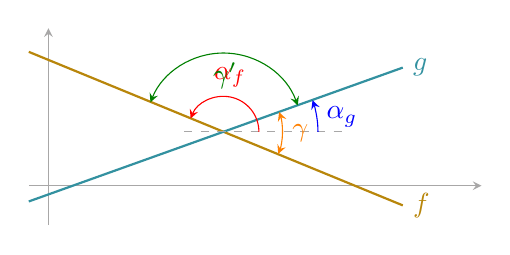
\begin{tikzpicture}[pfeil]

    % \draw[thick, fill=petrol!20, draw=petrol-lighter, rounded corners=2ex, opacity=0.5] (0,0) rectangle ++ (1.5,3.5);
    % \draw[thick, fill=darkgoldenrod!20, draw=darkgoldenrod-lighter, rounded corners=2ex, opacity=0.5] (5,0) rectangle ++ (1.5,3.5);

    \draw[-stealth] (-0.25,0) -- (5.5,0);
    \draw[-stealth] (0,-0.5) -- (0,2);
    \draw[thick, darkgoldenrod, name path=F] (-0.25,1.7) -- (4.5,-0.25) node[right] {$f$};
    \draw[thick, petrol-light, name path=G] (-0.25,-0.2) -- (4.5,1.5) node[right] {$g$};
    
    % \coordinate (S) at (2.3409,0.6590878756);
    \path [name intersections={of=F and G,by=S}];
    
    \draw[thin,dashed] (S) ++ (-0.5,0) -- ++ (2,0);
    
    
    \draw[red,-stealth] (S) ++ (0.45,0) arc (0:79:0.45) node[above]{$\alpha_f$} 
        arc (79:158:0.45);
    \draw[blue,-stealth] (S) ++ (1.2,0) arc (0:9:1.2) node[right]{$\alpha_g$} 
        arc (9:19.5:1.2);
    \draw[green!50!black,stealth-stealth] (S) ++ (19.5:1) arc (19.5:89:1) node[below] {$\gamma'$} 
        arc (89:158:1);
    \draw[orange,stealth-stealth] (S) ++ (-22:0.75) arc(-22:-1:0.75) node[right] {$\gamma$} 
        arc(-1:19.5:0.75);
    

\end{tikzpicture}

\end{document}
